\documentclass[10pt]{beamer}

\usetheme{metropolis}
\usepackage{appendixnumberbeamer}

\usepackage{outlines}

\title{HPX Backend for Blaze}
%\subtitle{}
\author{Shahrzad Shirzad}
\date{Nov 7, 2019}
%\institute{Division of Computer Science and Engineering \\ School of Electrical Engineering and Computer Science \\ Louisiana State University}
\titlegraphic{
\includegraphics[height=10mm]{logos/stellar_4x1.pdf}}
\titlegraphic{
	\begin{tikzpicture}[overlay, remember picture]
	\node[at=(current page.south east), anchor=south east] {%
		
\includegraphics[width=.25\textwidth]{logos/stellar_4x1.pdf} 
	};
%	\node[at=(current page.south west), anchor=south west] {%
%		
\includegraphics[width=.50\textwidth]{logos/cct_logo.pdf} 
%	};
	\end{tikzpicture}
}


\begin{document}
\setbeamercolor{background canvas}{bg=white}
\maketitle

%\begin{frame}{Outline}
%  \setbeamertemplate{section in toc}[sections]
%  \tableofcontents[hideallsubsections]
%\end{frame}

%\section{Introduction}

\begin{frame}{Blaze}
\begin{outline}
 Linear Algebra Library based on Smart Expression Templates
 \1Expression Templates:
	\2Creates a parse tree of the expression at compile time and postpone the actual evaluation to when the expression is assigned to a target
\1 Smart: 
	\2Creation of intermediate temporaries when needed
	\2Integration with highly optimized compute kernels
\end{outline}
\end{frame}


\begin{frame}{Parallelization}
	\begin{outline}
		Depending on the operation and the size of operands, the assignment could be parallelized through four different backends
		\1 HPX 
		\1OpenMP
		\1C++ threads
		\1Boost
	\end{outline}
\end{frame}

\begin{frame}{HPX Backend}
	\begin{outline}
		In the current implementation the work is equally divided between the cores at compile time.
		\1 HPX for-loop with static chunking and chunk size=1
		\begin{figure}
			\centering
			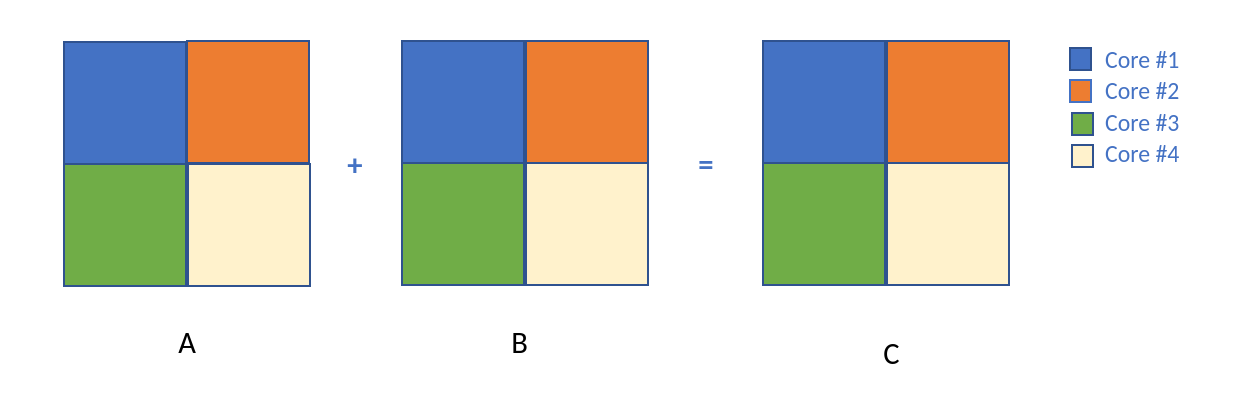
\includegraphics[width=0.72\linewidth]{figures/old_backend.png}
			\caption{An example of how C=A+B is performed in HPX Backend with 4 cores}	
		\end{figure}	

	\end{outline}
\end{frame}

\begin{frame}{Objective}
	\begin{outline}
		Dynamically divide the work among the cores based on number of cores, matrix size, operation, etc.
		For this purpose two parameters have been introduced:
		\1block\textunderscore size: at each loop iteration the assignment is performed on one block
		\1chunk\textunderscore size: the number of loop iterations included in one task 
		\begin{figure}
			\centering
			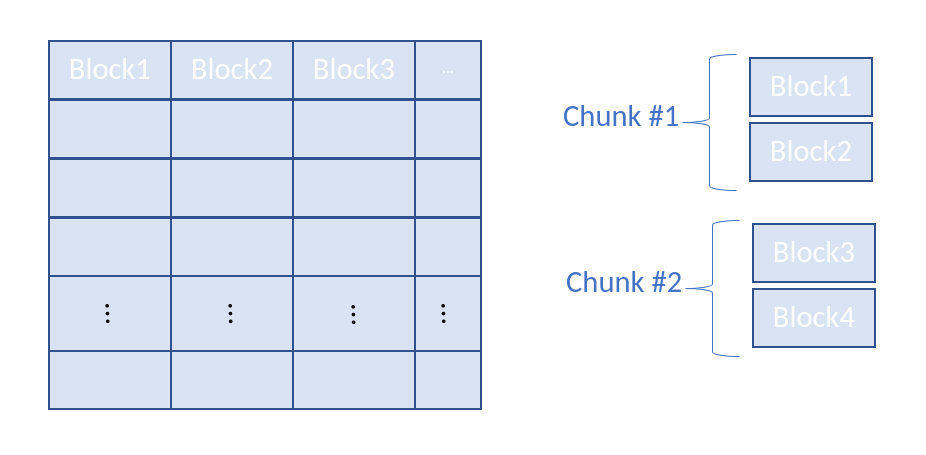
\includegraphics[width=0.72\linewidth]{figures/chunks.png}
			\caption{An example of blocking and creating chunks for chunk\textunderscore size = 2}	
		\end{figure}	
	\end{outline}
\end{frame}


\begin{frame}{Background}
	\begin{outline}
		\1 Effect of Task Granularity on execution time
		\1 Universal Scalibility Law
	\end{outline}
\end{frame}


\begin{frame}{Task Granularity}
	\begin{outline}
		Grain size: The amount of work performed by one HPX thread
		\begin{figure}
			\centering
			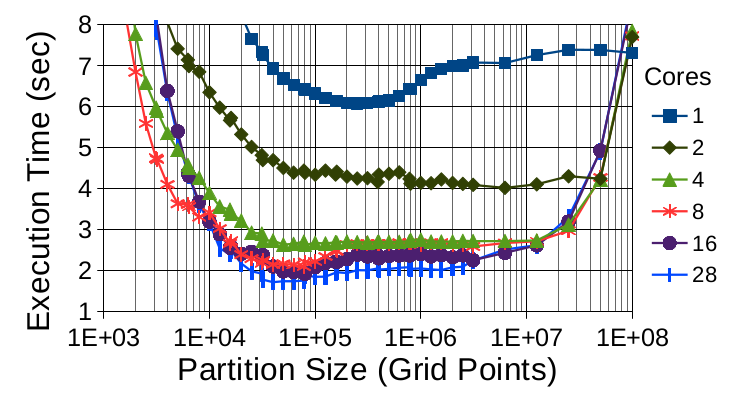
\includegraphics[width=0.72\linewidth]{figures/task_granularity.png}
			\caption{The effect of task size on execution time for Stencil application\footnote{Grubel, Patricia, et al. "The performance implication of task size for applications on the hpx runtime system." 2015 IEEE International Conference on Cluster Computing. IEEE, 2015.}}	
	
		\end{figure}
		
	\end{outline}
\end{frame}

\begin{frame}{Universal Scalibility Law}
	\begin{outline}
		\1 Models the effects
		of linear speedup, contention delay, and coherency delay due to crosstalk
		\begin{figure}
			\centering
			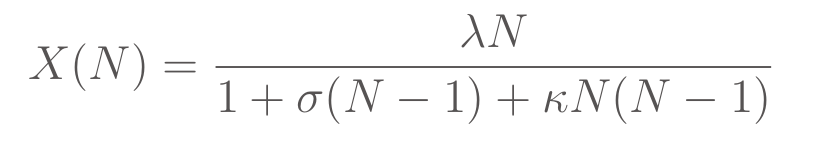
\includegraphics[width=0.5\linewidth]{figures/usl_formula.png}
			
			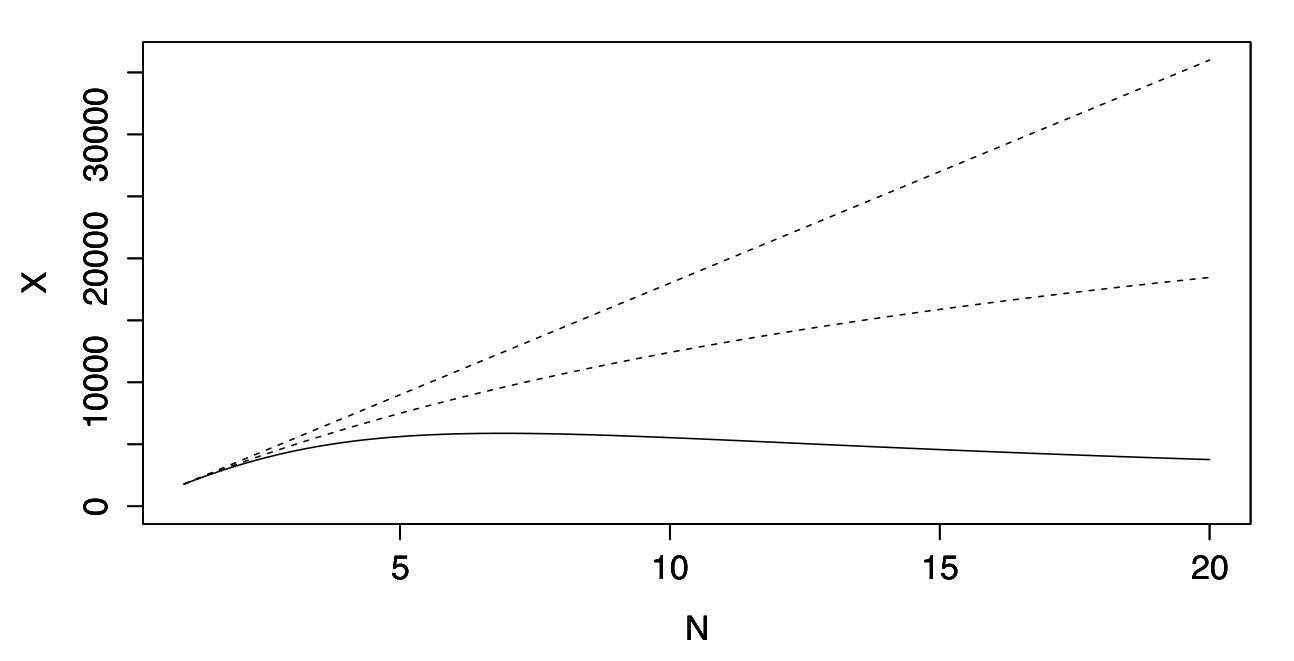
\includegraphics[width=0.72\linewidth]{figures/usl.png}
			\caption{Throughput vs. number of cores\footnote{Schwarz, B. "Practical Scalability Analysis with the Universal Scalability Law." (2015).}}				
		\end{figure}

	\end{outline}
\end{frame}

\begin{frame}{Blazemark}
	\begin{outline}
		Blazemark is a benchmark suite provided by Blaze to compare the performance of Blaze with other linear algebra libraries. 
		\begin{figure}
			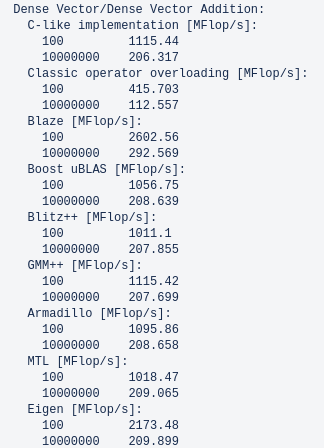
\includegraphics[width=0.42\linewidth]{figures/blazemark_1.png}
			\hfill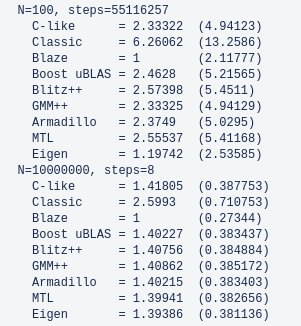
\includegraphics[width=0.41\linewidth]{figures/blazemark_2.png}
			\caption{An example of results obtained from Blazemark}	
		\end{figure}
	\end{outline}
\end{frame}

\begin{frame}{Method}
	\begin{outline}
	\1 Starting from \textit{DMATDMATADD} benchmark, C = A + B where A, B, and C are N by N matrices
	\1 Collect data with different configurations such az matrix size, number of cores, block\textunderscore size, chunk\textunderscore size. 
		\2matrix sizes: 200, 230, 264, 300, 396, 455, 523, 600, 690, 793, 912, 1048, 1200, 1380, 1587
		\2number of cores: 1, 2, 3, ..., 8
		\2block\textunderscore{sizes}: {[4, 8, 12, 16, 20, 32]} by {[64, 128, 256, 512, 1024]} blocks
		\2chunk\textunderscore{sizes}: between 1 and total number of blocks (logarithmic increase)
	\end{outline}
\end{frame}

\begin{frame}{Results}
	\begin{outline}
		\begin{figure}
			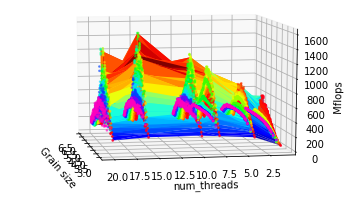
\includegraphics[width=0.9\linewidth]{figures/grain_size_marvin_color.png}	
			\caption{Results of running the \textit{DMATDMATADD} benchmark for different matrix sizes with different block\textunderscore{size} and chunk\textunderscore{size} combinations}	
		\end{figure}
	\end{outline}
\end{frame}

\begin{frame}{Method}
	\begin{outline}
			\begin{figure}
			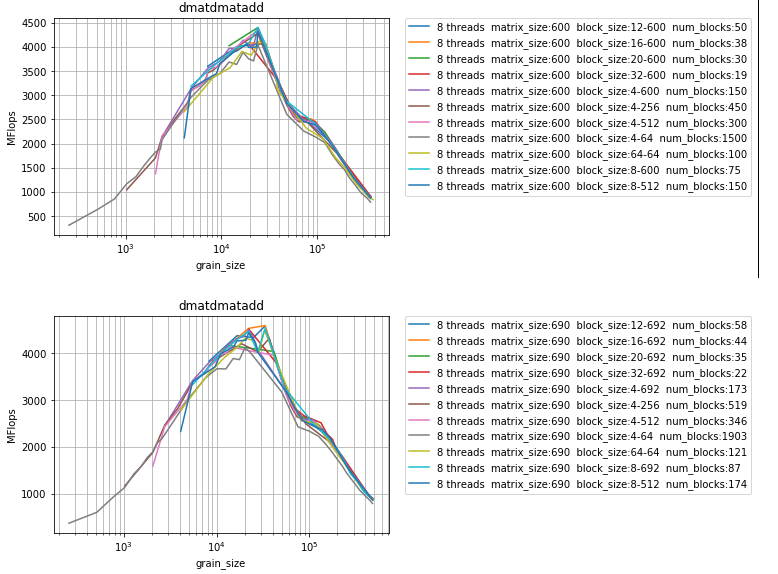
\includegraphics[width=0.9\linewidth]{figures/mflop_2.png}	
			\caption{Results of running the \textit{DMATDMATADD} benchmark on 8 cores for different block sizes}	
		\end{figure}
	\end{outline}
\end{frame}

\begin{frame}{Modeling Execution Time based on Grain Size}
	\begin{outline}
		\begin{figure}
			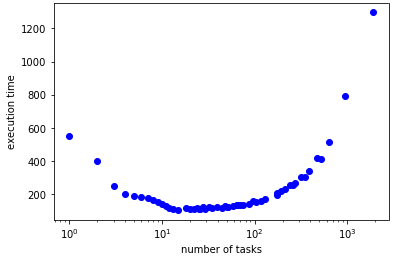
\includegraphics[width=0.9\linewidth]{figures/true_1.png}	
			\caption{Results of running the \textit{DMATDMATADD} benchmark on 8 cores matrix size 690(time unit is microseconds)}	
		\end{figure}
	\end{outline}
\end{frame}

\begin{frame}{Modeling Execution Time based on Grain Size}
	\begin{outline}		
		\1Overheads of creating tasks
		\1Starvation
		\begin{figure}
			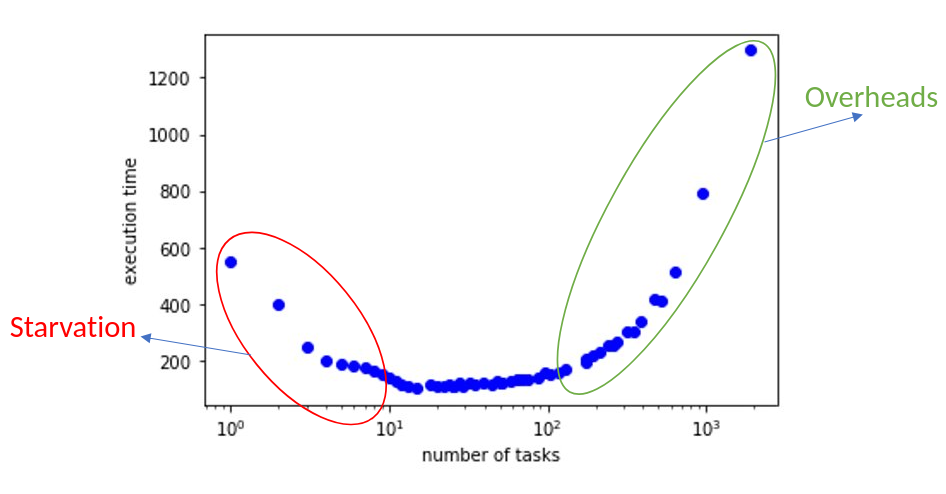
\includegraphics[width=0.9\linewidth]{figures/true_1_annotated.png}	
			\caption{Results of running the \textit{DMATDMATADD} benchmark on 8 cores matrix size 690(time unit is microseconds)}	
		\end{figure}
	\end{outline}
\end{frame}

\begin{frame}{Modeling Execution Time based on Grain Size}
\begin{outline}		
	\begin{figure}
		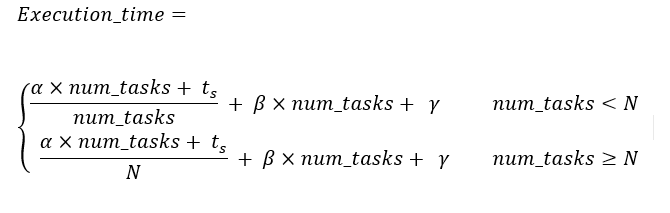
\includegraphics[width=0.9\linewidth]{figures/formula.png}			
	\end{figure}
\end{outline}
\end{frame}

\begin{frame}{Modeling Execution Time based on Grain Size}
\begin{outline}	
	\1Fixed matrix size, and number of cores	
	\1Training set and test set (\%60, \%40)
	\begin{figure}
		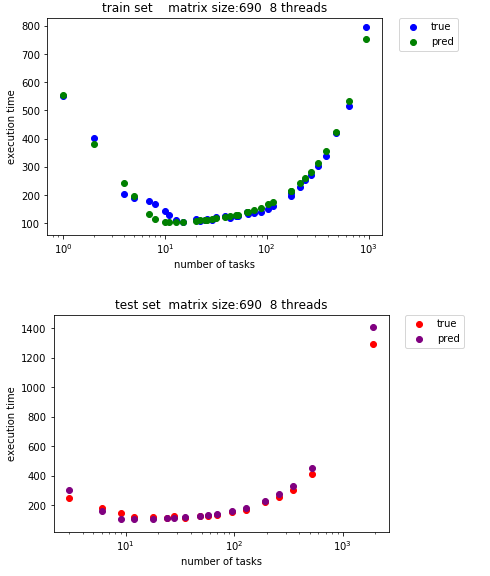
\includegraphics[width=0.6\linewidth]{figures/pred_1.png}	
		\caption{Results ofpredicting execution time )}	
	\end{figure}
\end{outline}
\end{frame}

\begin{frame}{Modeling Execution Time based on Grain Size}
\begin{outline}	
	\1For a fixed matrix size, and number of cores we need 4 parameters to estimate execution time based on number of tasks
    \1How does these four parameters change for different number of cores?
    \2used USL to model each of these parameters
\end{outline}
\end{frame}

\begin{frame}{Modeling Execution Time based on Grain Size}
\begin{outline}	
	
	\begin{figure}
		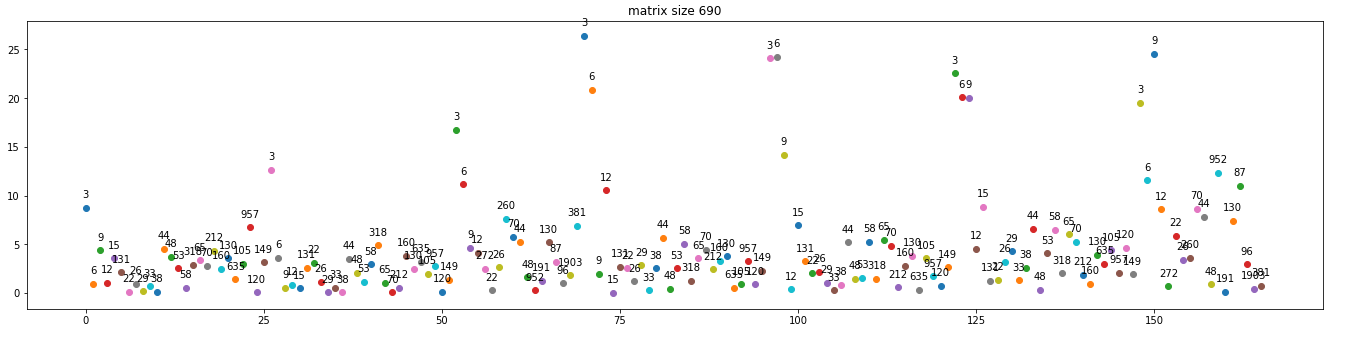
\includegraphics[width=1\linewidth]{figures/error.png}	
		\caption{Relative error of predicting execution time}	
	\end{figure}
\end{outline}
\end{frame}

\begin{frame}{Next Step}
\begin{outline}	
	\1Find the range of the flat region of grain size  
	\1Choosing a small block\textunderscore{size} while number of columns is divisible by cache line
	\1Find the range of chunk\textunderscore{sizes} for the given range of grain size
	\1Generalize the model to integrate the matrix size 
\end{outline}
\end{frame}


\begin{frame}[standout]
  Thank you!
\end{frame}

\end{document}
